%% The following is a directive for TeXShop to indicate the main file
%%!TEX root = diss.tex

\chapter{Entropy in mesoscopic systems}
\label{ch:Theory}

In this chapter, we review the theoretical underpinnings for the measurements that were completed. First, we discuss some of the theory behind single and double quantum dots and the relevant energy scales for these systems. We then proceed to a review of entropy in quantum systems, finally discussing the Maxwell relation used to make the measurements of entropy presented in this thesis and those presented by Hartman et al.

\section{Entropy of quantum systems}
The classical description of entropy comes in the form of the Boltzmann entropy
\begin{equation}
	\label{eqn:b_entropy}
	S = k_b \ln W.
\end{equation}
Here, $W$ is defined by the number of available microstates of the system \cite{schroeder}. In the context of simple quantum systems at $T$ close to zero (such that excited states are unattainable), it is useful to consider this quantity, $W$, as the degeneracy, $d$, of the ground state of the system~\cite{mcquarrie}. 

As a simple example, and closely related to the results from this thesis, consider a single potential well that may be occupied by some small number of electrons as illustrated in Fig~\ref{fig:potential_wells} (a).  In the example outlined Fig~\ref{fig:potential_wells} (a), the possible occupations, $n$, of the well are shown. This system can also be thought of, very approximately, as a model for a single atom with excited states unreachable at low enough $T$~\footnote{In practice, potential wells like this can be fabricated on a mesoscopic scale -- much larger than any atom -- to study the behavior of electrons in ``artificial" atoms cf. Ch. ~\ref{ch:Methods}. These structures are called quantum dots.}. In the $n = 0$ state the system has no degeneracy since there is only one state at ground state energy -- no electrons anywhere. However, in the $n=1$ state, the system develops a ground state degeneracy of $d = 2$ since the single electron will be in either a spin up or spin down state, both of which will be of the same energy. Finally, if a second electron is added to the system, the spin degeneracy of the system will break as the lowest energy state of the pair of electrons will be a spin singlet state disallowing net spin freedom of the system. 

One can consider the change in entropy, $\Delta S$, of a given transition in the occupation of the potential well\footnote{For now, where this electron came from will be neglected.} like the transition from $n = 0 \to n = 1$ as shown in Fig~\ref{fig:potential_wells} (b). For this transition, $\Delta S = k_B \ln d_f - k_B \ln d_i = k_B \ln 2$ by Eqn.~\ref{eqn:b_entropy}.
\begin{figure}[h]
\centering
\resizebox{1\textwidth}{!}{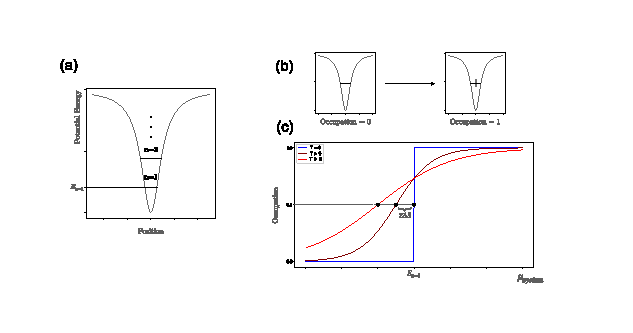
\includegraphics{figures/pdfs/quantum_well_theory.eps}}
\caption{In (a) a simple potential well is shown, with the energy levels of various occupations plotted on top of the potential diagram. In (b) and (c) a transition from $0 \to 1$ electrons in the potential well is illustrated. In (c) finite temperature broadening of this transition, as well as a shift in $\mu_{system}$, due to the change in entropy of the transition, is shown as temperature increases (still much too small to allow for excited states). }
\label{fig:potential_wells}       % Give a unique label to the figure. 
\end{figure}

Next, we consider the energy at which such a transition would occur, labelled as $E_{n=1}$ for $T=0$. As temperature is increased, the chemical potential of the system, $\mu_{system}$, at the ``half-occupancy" point of such a transition will be affected by the $\Delta S$ of the system due to the effect that entropy has on the Helmoltz free energy, $F$, of a given configuration.
\begin{equation}
	F = E - T \Delta S \quad \to \quad \mu_{sys, transition}  = E_{n=1} - T \Delta S
\end{equation}
Graphically, this effect is shown in Fig~\ref{fig:potential_wells} (c), where in addition to an effective broadening of the transition from finite $T$, the ``half-occupancy" point of the transition from $0 \to 1$ electrons shifts in $\mu_{system}$. It is this affect which we have used in measurements in this thesis to quantify changes in entropy.

\section{From a Maxwell relation to entropy}
\label{sec:mrtoentropy}

The shift in the transition based on a change in entropy as summarized above can be quantified by the following Maxwell relation.

\begin{equation}
	\label{eqn:MR}
	\left( \frac{\partial \mu }{\partial T} \right)_{p,N} = -\left( \frac{\partial S}{\partial N} \right)_{p,T}
	%\Delta S = \int_{\mu_1}^{\mu_2} \frac{dN(\mu)}{dT}\,\, d\mu
\end{equation}


Qualitatively, this relation tells us that the change in entropy over the course of a transition in $N$ (e.g. from some $N$ to $N+1$ particles in a given system) can be expressed in terms of the shift of that transition (in chemical potential) as a function of temperature. As with all the Maxwell relations, there are is an additional constant-variable requirement -- pressure, $p$, cannot vary -- which will be discussed further in Ch.~\ref{ch:Methods}. To further illustrate this qualitative explanation, consider an integral form of the above relation.

\begin{equation}
	\label{eqn:MRintegral}
	\Delta S = - \int_{\mu_1}^{\mu_2} \frac{dN(\mu)}{dT}\,\, d\mu
\end{equation}

In other words, by measuring the occupation of a system as a function of the chemical potential, $N(\mu)$, and varying temperature, $T$, one can derive the change in entropy, $\Delta S$ over that change in occupation. 

In Fig.~\ref{fig:potential_wells}, the change in entropy was related to a shift in the mid point of the occupation (of the system) as a function of chemical potential or $N(\mu)$ curve. This shift can also be thought of in terms of the change it would induce in Eqn.~\ref{eqn:MRintegral}. If one considers the approximate $dN/dT$ by looking at the difference between a `warmer' and `colder' curve in the figure, it can be noted that, if there is no shift in the center, $\frac{dN}{dT} (\mu)$ will be exactly antisymmetric and therefore integrate to 0. Whereas, in the case that is illustrated, this approximate $\frac{dN}{dT} (\mu)$  is not exactly antisymmetric and will integrate to a finite value.

\section{Approximate form for a quantum dot coupled to a thermally broadened lead}

\begin{equation}
	\label{eqn:occupation}
	N(\mu, \Theta) = 
\end{equation}

\begin{equation}
	\label{eqn:dndt}
	d
\end{equation}

\endinput

Any text after an \endinput is ignored.
You could put scraps here or things in progress.
